\section{Matrix Factorization Visualization}

For each movie \textit{j} we visualize it as a 2D vector using the coordinates $\bar{V}[1:2,j]$, where $\bar{V}$ is obtained from the previous section. We show 10 random movies in Figure~\ref{fig:tenRandom}, the most popular 10 movies in Figure~\ref{fig:tenMostPopular} and the best 10 movies in Figure~\ref{fig:tenBest}. We observe that similar movies are closer together but in general there is no correlation between distance in the plots and movie similarity as seen by the authors. \\
The observe that the most popular 10 movies are located along the line $(1,1)$ while the best 10 movies cover the 2D space more uniformly .
Figure~\ref{fig:tg} shows the representation for the genres horror, children and fantasy. The movies withing each genre tend to cluster together but the variance for each genre is very high as it can be seen in .

\begin{figure}[hptb]
\centering
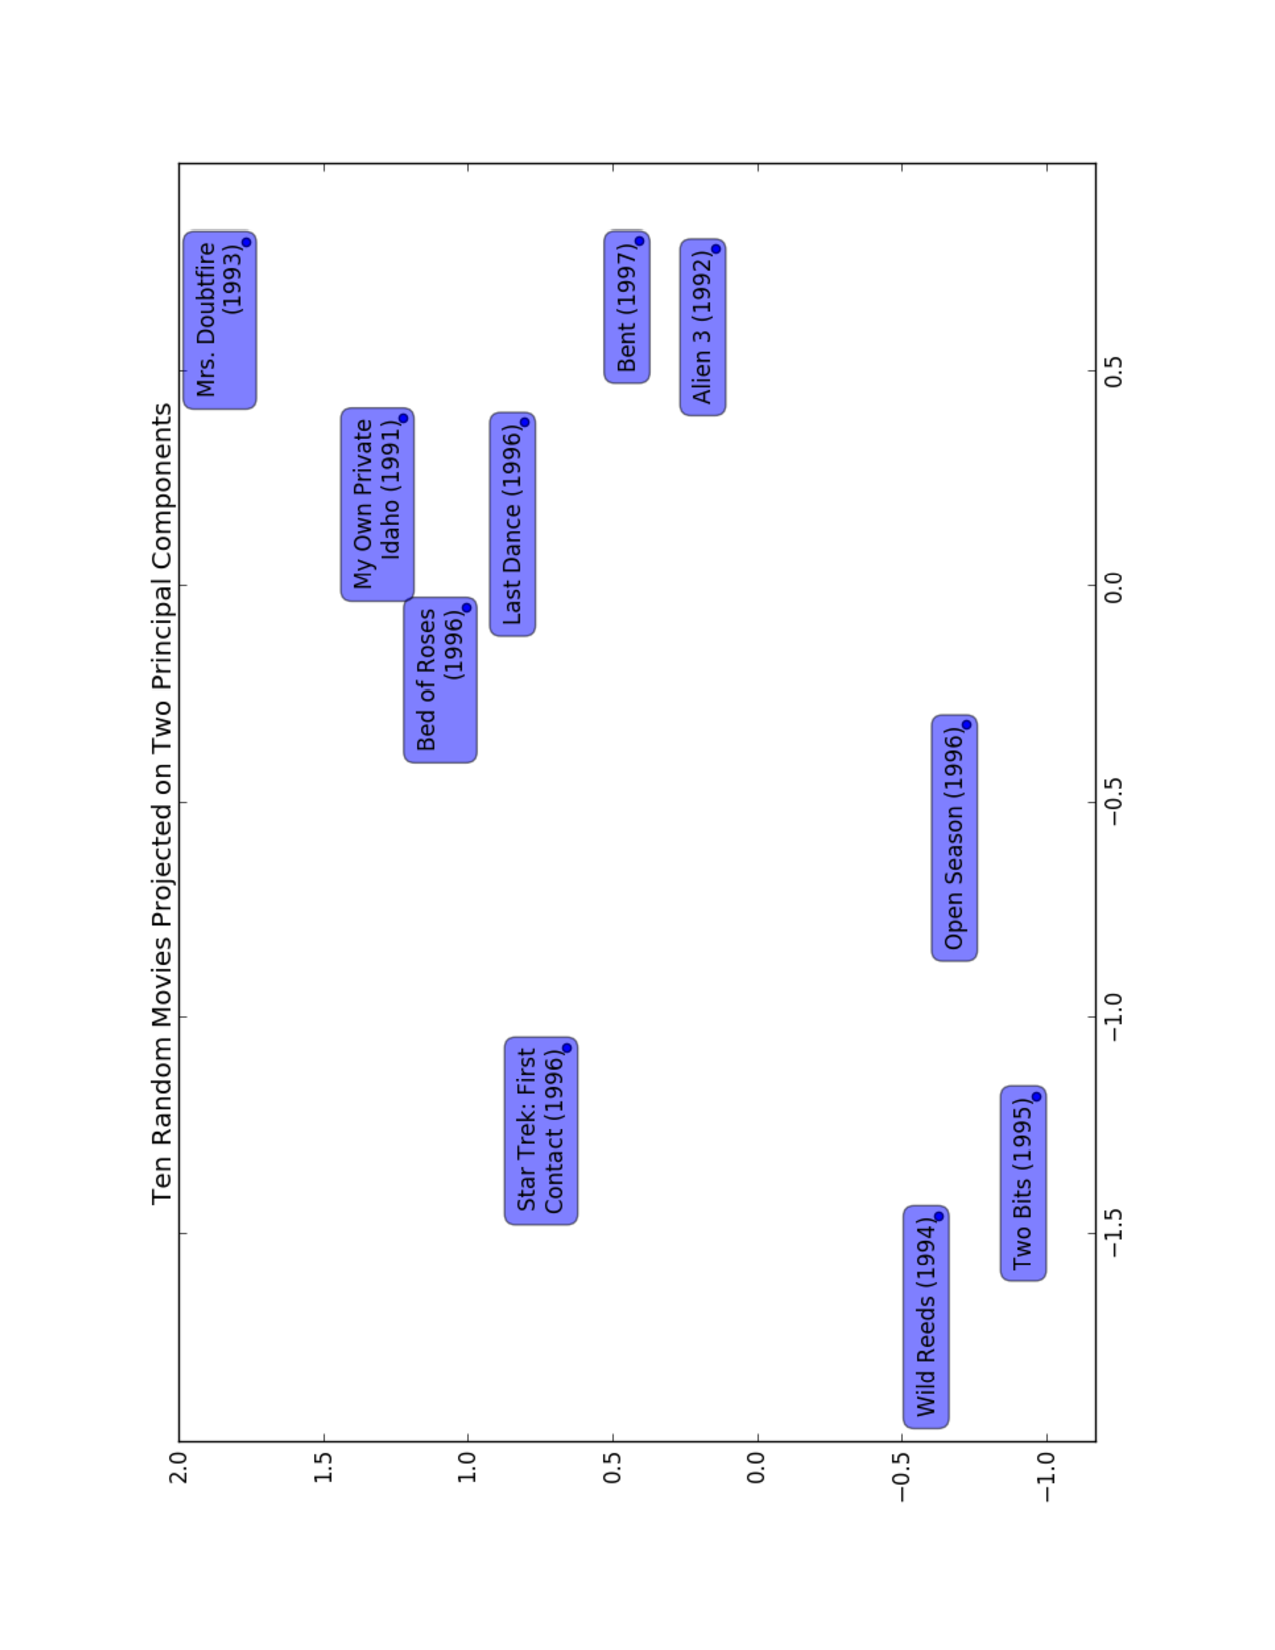
\includegraphics[width=0.8\textwidth, angle =270]{Random_10_Movies.pdf}
 \caption{Ten Random movies projected along two principal components.}
\label{fig:tenRandom}
\end{figure}


\begin{figure}[hptb]
\centering
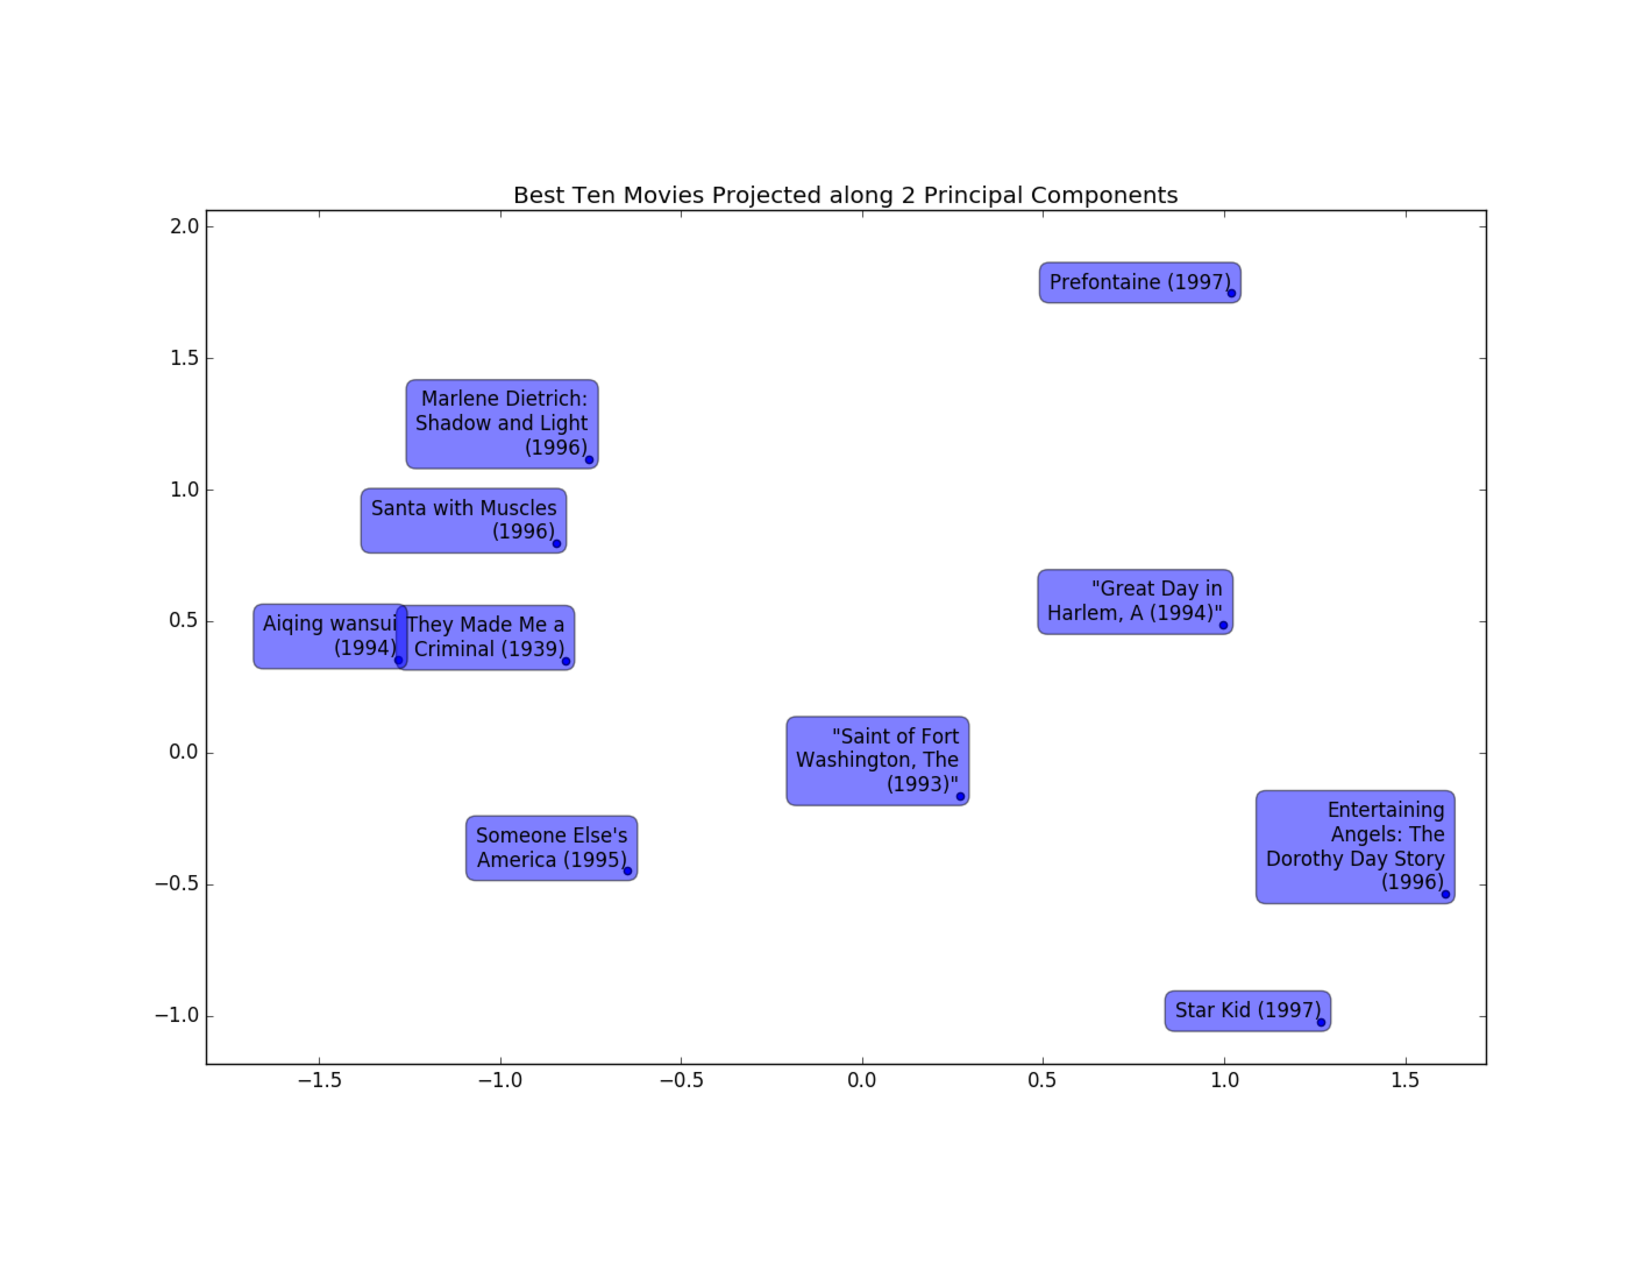
\includegraphics[width=0.8\textwidth, angle = 270]{Best_10_Movies.pdf}
 \caption{Best ten movies projected along two principal components.}
\label{fig:tenBest}
\end{figure}


\begin{figure}[hptb]
\centering
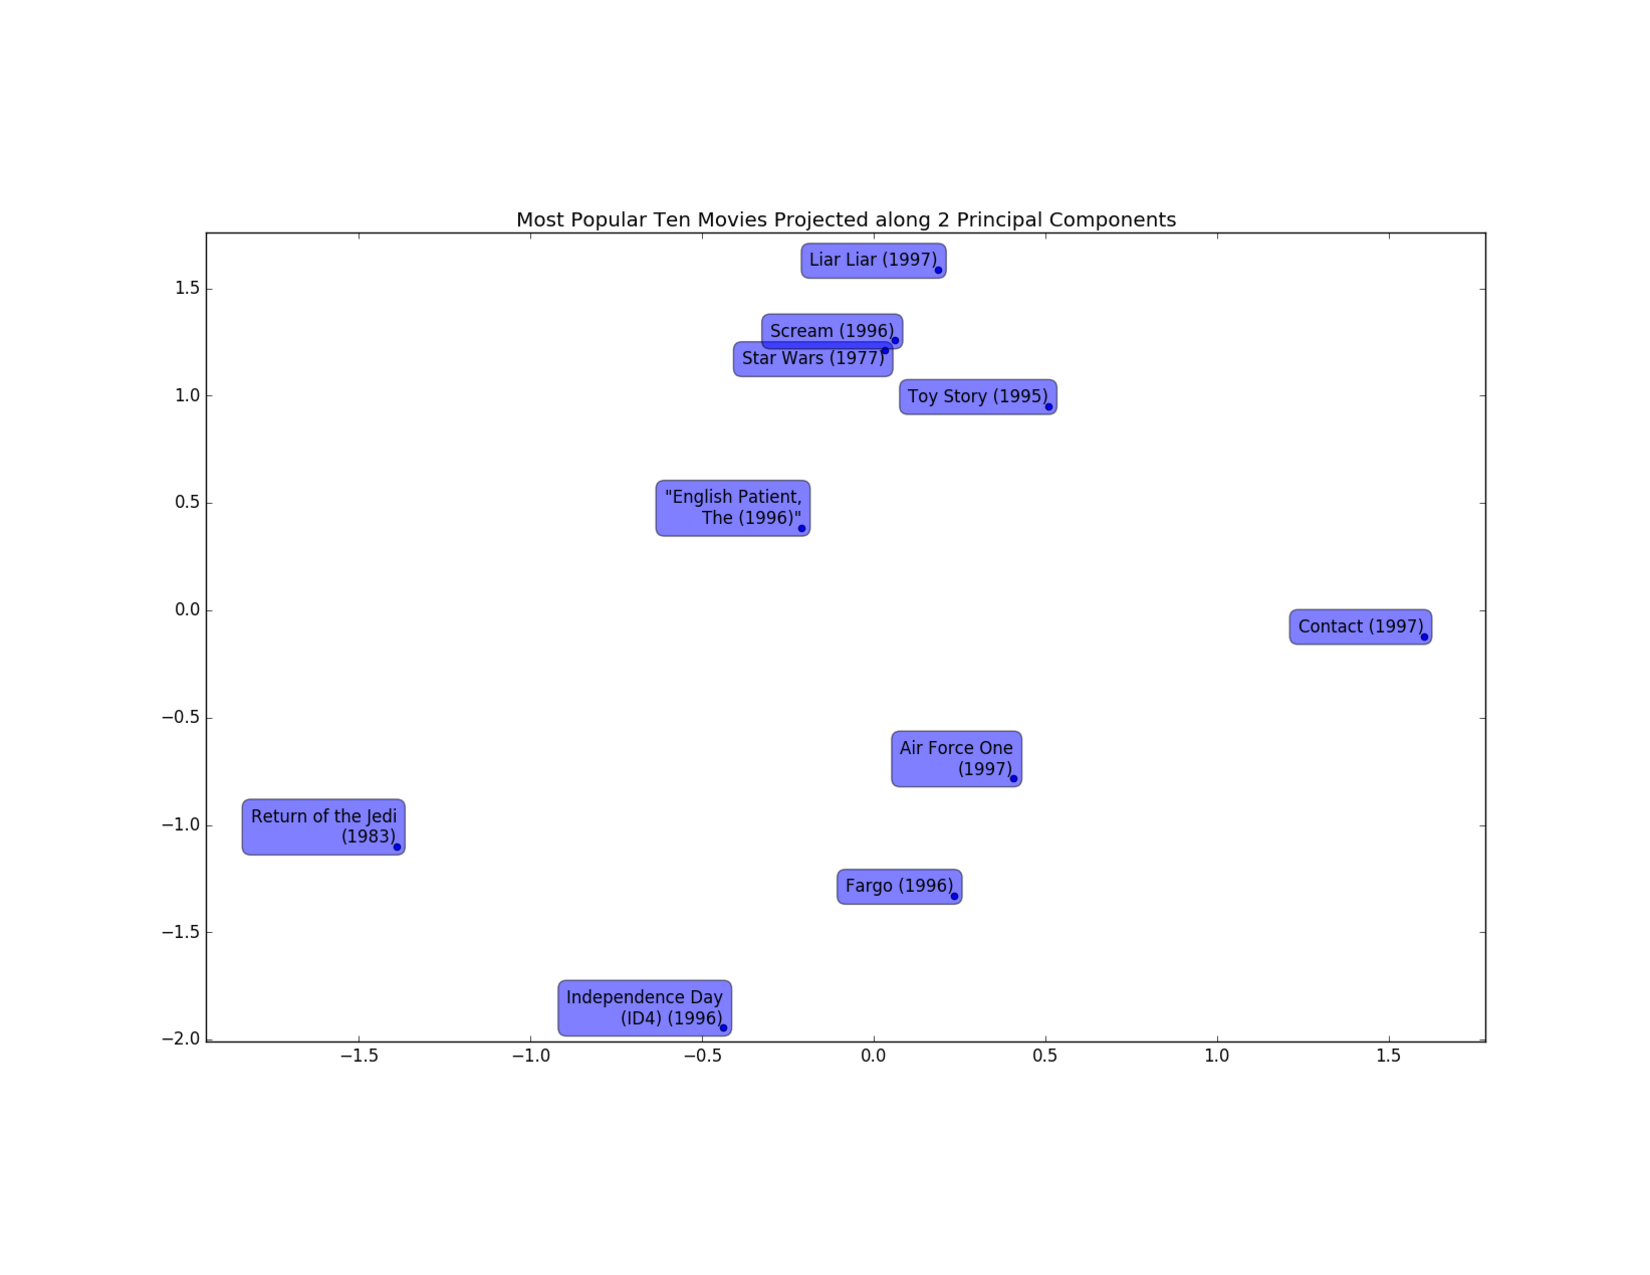
\includegraphics[width=0.8\textwidth, angle =270]{Popular_10_Movies.pdf}
 \caption{Most popular ten movies projected along two principal components.}
\label{fig:tenMostPopular}
\end{figure}


\begin{figure}[hptb]
\centering
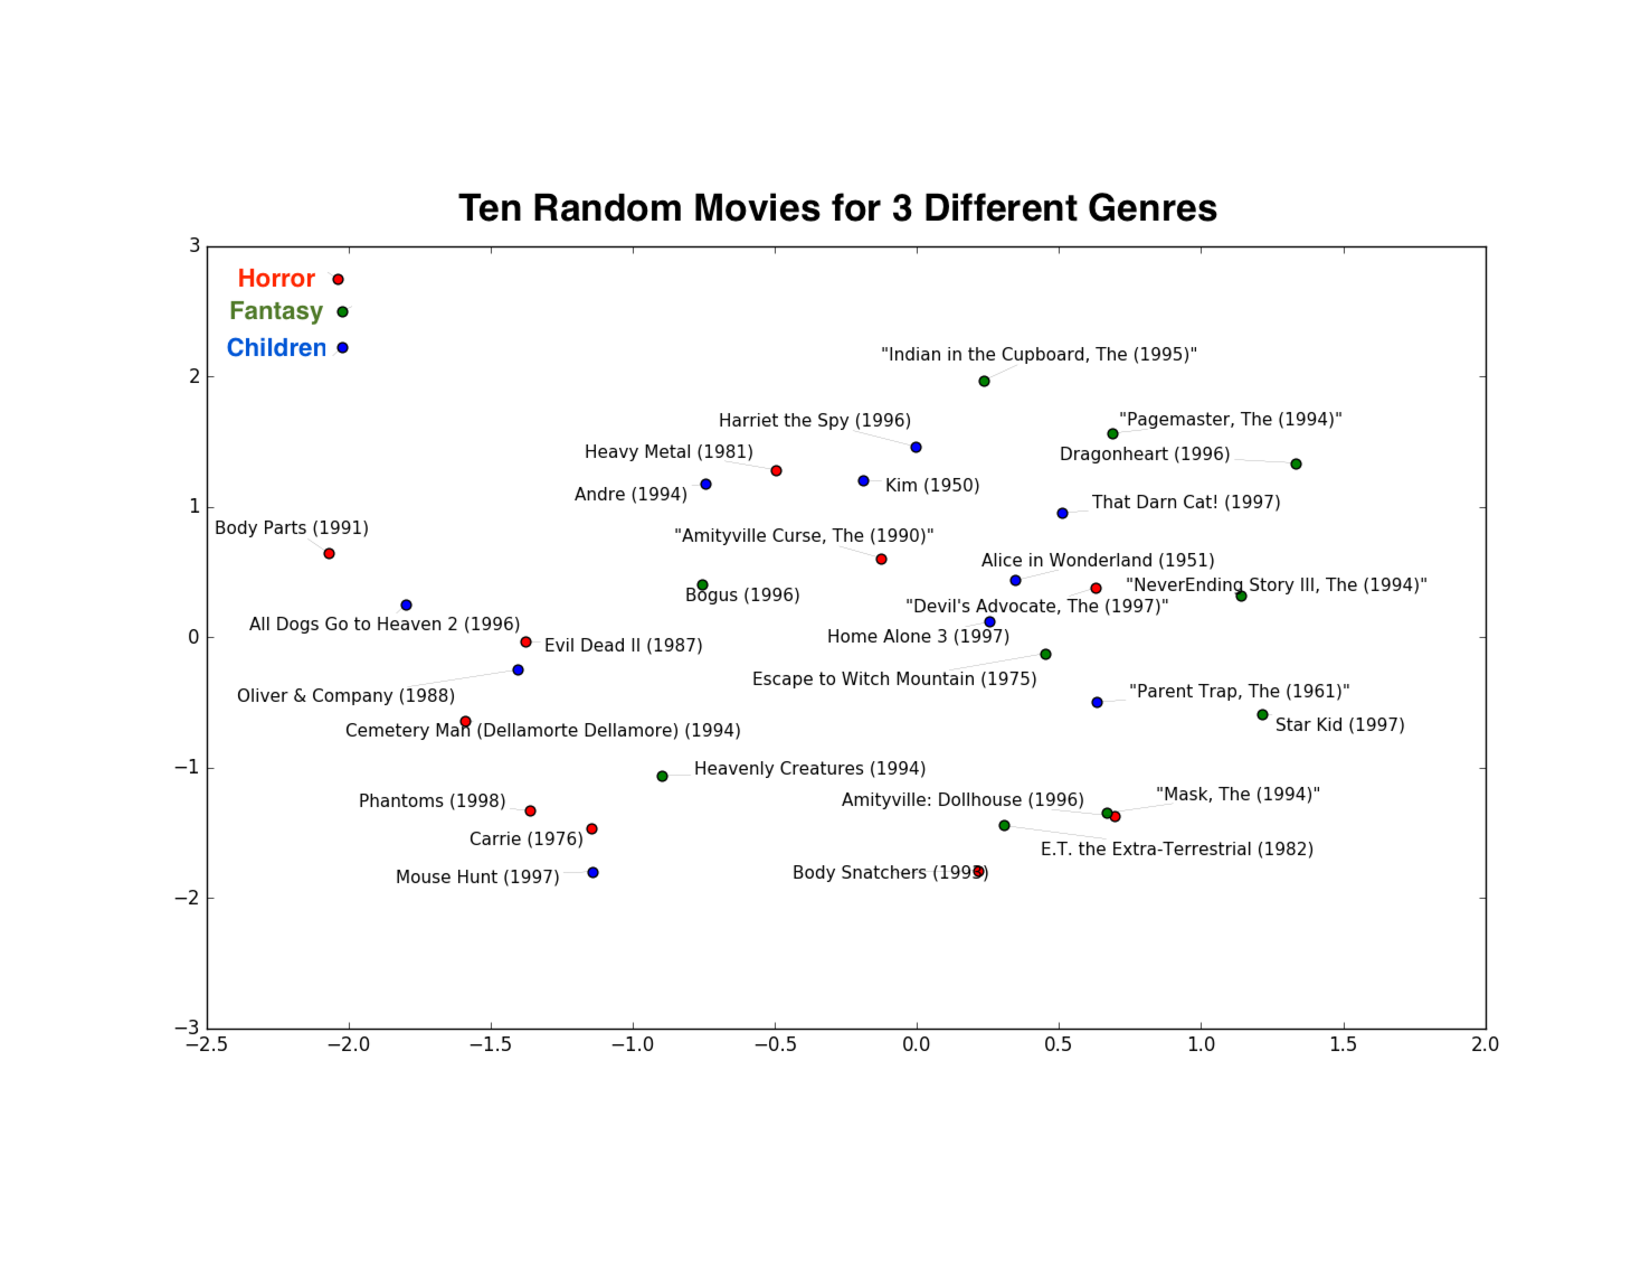
\includegraphics[width=0.8\textwidth, angle =270]{Three_Genres.pdf}
 \caption{ }
\label{fig:tg}
\end{figure}